\documentclass[12pt]{amsart}
\pagestyle{empty}
\usepackage{array}
\usepackage{amsmath}
\usepackage{subcaption}
\usepackage{graphicx}


\title{A Stochastic Spatial Model for Tumor Growth}
\author{Aashiq Dheeraj, Rick Durrett}

\begin{document}
\maketitle

\section{Figures}
\begin{figure}[ht]

	\begin{subfigure}[b]{0.5 \textwidth}
		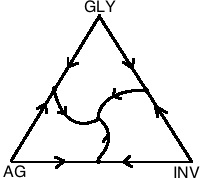
\includegraphics[width = 0.4\textwidth]{Diagrams/Basanta/phase}
		\caption{Phase Portrait has attracting fixed point, implying coexistence}
	\end{subfigure}
	~~~
	\begin{subfigure}[b]{0.5 \textwidth}
		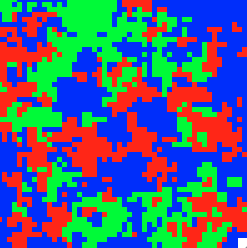
\includegraphics[width = 0.4 \textwidth]{Diagrams/Basanta/sample}
		\caption{Sample Output. Cells of type AG are red, INV green and GLY blue.}
	\end{subfigure}

\caption{if this works...}
\end{figure}

\end{document}